% !TeX root = ..\rapport_13_2.tex
\section{Programstruktur}\label{sec:struct}
\subsection{Import af program som projekt}
\subsubsection{Eclipse}
\subsubsection{IntelliJ}
\subsubsection{VS Code}

\subsection{Start af programmet}
For at kører TaskFusion, skal følgende fil køres: \texttt{TaskFusion/src/main/taskFusion/cli/TaskFusionCLI.java}
Ingen kodeord er nødvendige for at kører programmet.
Programmet kommer med demo-data installeret. Du kan derfor logge ind med følgende initialer; \texttt{kasy}, \texttt{rawi}, \texttt{mach}, \texttt{mash}.

\subsection{Mappe struktur}
\cref{fig:tree} viser mappestrukturen i Java projektet.
\begin{figure}[H]
    \caption{Mappestrukturen i Java projektet TaskFusion}\label{fig:tree}
    \dirtree{%
        .1 TaskFusion \ldots{} \begin{minipage}[t]{10cm} Rodmappe til filer som \emph{pom.xml}, \emph{.project} and \emph{.classpath} \end{minipage}.
        .2 features \ldots{} \begin{minipage}[t]{5cm} Cucomber feature filer \end{minipage}.
        .2 src.
        .3 main.
        .4 java.
        .5 taskfusion \ldots{} \begin{minipage}[t]{5cm} \mintinline{java}|.java| filer \end{minipage}.
        .6 app.
        .6 domain \ldots{} \begin{minipage}[t]{5cm} Domæne-lag \end{minipage}.
        .6 exceptions \ldots{} \begin{minipage}[t]{5cm} Exception klasser \end{minipage}.
        .6 helpers \ldots{} \begin{minipage}[t]{5cm} Diverse hjælper klasser \end{minipage}.
        .6 persistency \ldots{} \begin{minipage}[t]{5cm} Lagrings-lag \end{minipage}.
        .6 viewModels \ldots{} \begin{minipage}[t]{5cm} Visningsklasser \end{minipage}.
        .6 facades \ldots{} \begin{minipage}[t]{5cm} Facade-lag \end{minipage}.
        .6 cli \ldots{} \begin{minipage}[t]{5cm} CLI brugergrænse-lag \end{minipage}.
        .7 controllers \ldots{} \begin{minipage}[t]{5cm} Menu controllere \end{minipage}.
        .7 views \ldots{} \begin{minipage}[t]{5cm} Indholdssider \end{minipage}.
        .7 components \ldots{} \begin{minipage}[t]{5cm} Genbrugelige CLI komponenter \end{minipage}.
        .7 TaskFusionCLI.java \ldots{} \begin{minipage}[t]{5cm} Hovedprogram ved brug af CLI brugergrænsefladen \end{minipage}.
        .3 test.
        .4 java.
        .5 taskfusion.
        .6 cucumber \ldots{} \begin{minipage}[t]{5cm} Acceptance tests \end{minipage}.
        .6 helpers \ldots{} \begin{minipage}[t]{5cm} Hjælpeklasser til tests \end{minipage}.
        .6 junit \ldots{} \begin{minipage}[t]{5cm} Unit tests \end{minipage}.
        .4 resources \ldots{} \begin{minipage}[t]{5cm} \emph{cucumber.properties} \end{minipage}.
    }
\end{figure}

\subsection{Program-lag}
Et klassediagram herunder i \ref{fig:class_persistency} viser relationer mellem klasserne i TaskFusion programmet. TaskFusion fungere som hovedklasse og er primært ansvarlig for brugergodkendelser. Sammen med \textit{EmployeeFacade} og \textit{ProjectFacade} eksponere \textit{TaskFusion} de offentlige metoder der skal kunne tilgås i programmet. På den måde kan vi frihed til at ændre alle metoder i de resterende program-lag, uden det vil påvirke eventuelle brugergrænseflader. Alle metoder i \textit{facade} klasserne kan i virkeligheden ligge i TaskFusion klassen, men ved at opdele metoderne i passende seperate klasser, kan vi bedre vedligeholde og udbygge programmet. 
Programmets domæne lag består af instantierbare objektklasser og er ansvarlig for \textit{Business-logic}. Persistency-laget indeholder \textit{Repositories}, der er ansvarlige for kommunikation med en lagringsløsning. Selvom programmet ikke har et database lag på nuværende tidspunkt, vil det være let at bygge flere lagringsløsninger på senere, ved kun at skulle modificere persistency klasserne. 
\\ \\
Vi ønsker desuden aldrig at eksponere programmets klasser udenfor program-laget. Derfor implementere alle instantierbare klasser \textit{ConvertibleToViewModel}-interfacet. Dette interface kræver at klasserne kan eksporteres til en tilsvarende visningsklasse til brug i præsentations-lag. 

\begin{figure}[H]
    \centering
    \caption{Klassediagram over program-laget}
    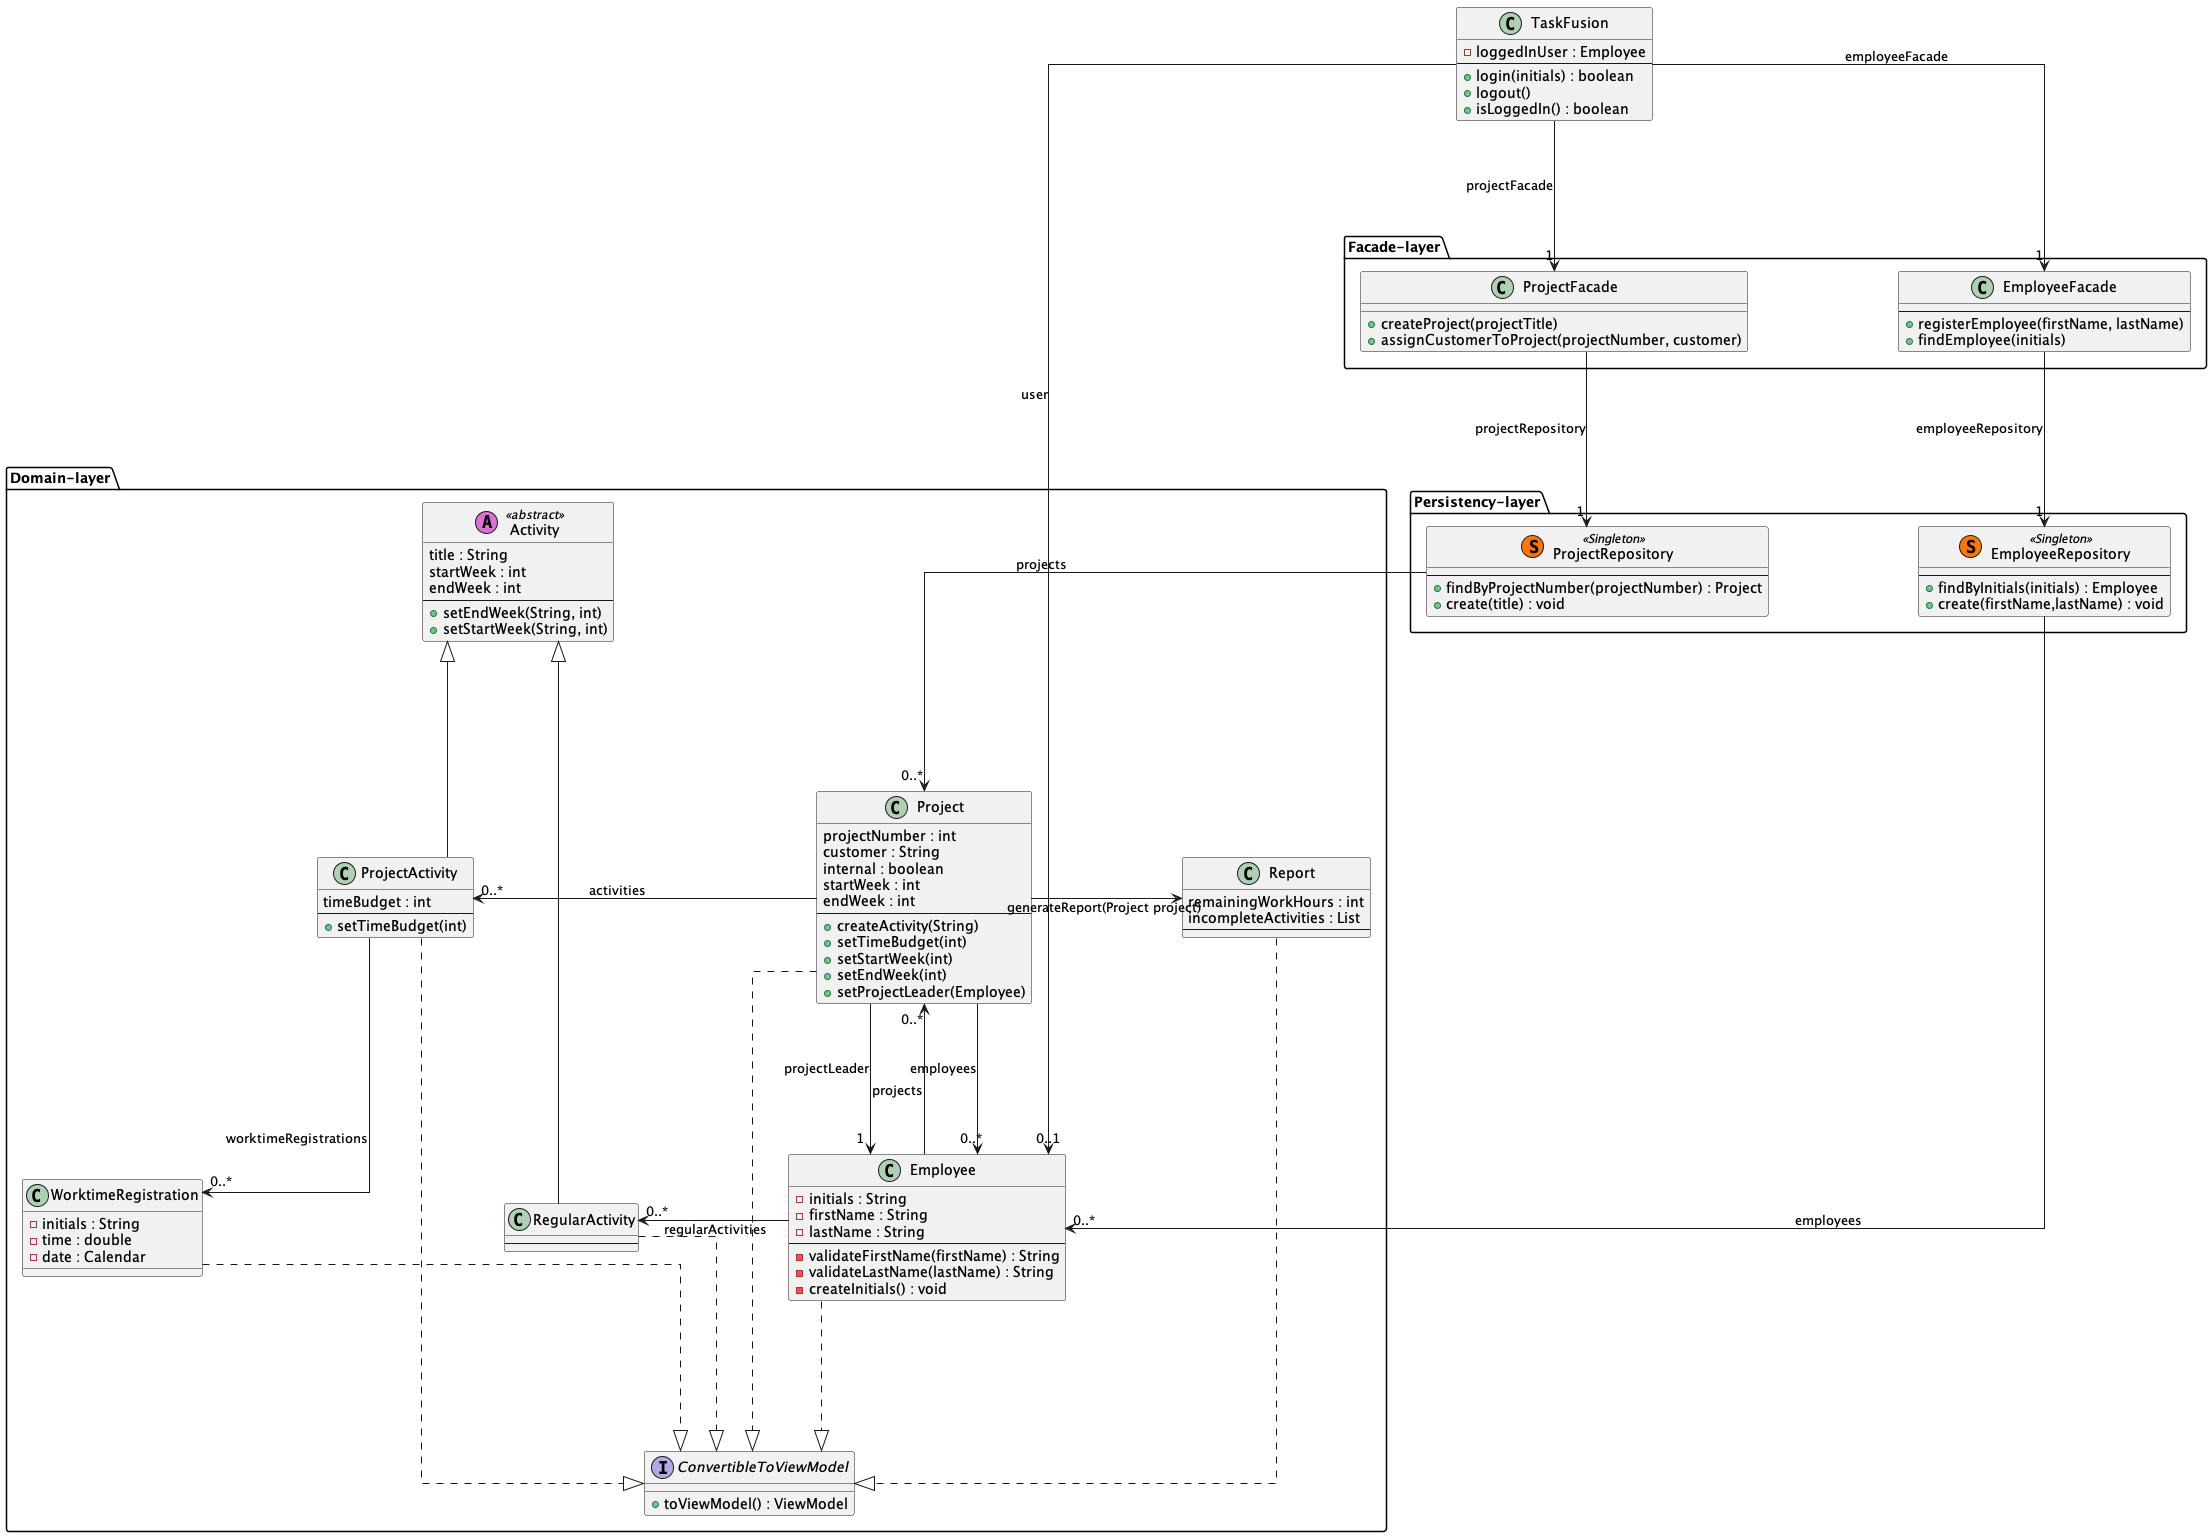
\includegraphics[width = \textwidth, keepaspectratio]{TaskFusion/out/assets/diagrams/class_persistency/ClassDiagram.png}
    \label{fig:class_persistency}
\end{figure}

\subsection{Præsentations-laget}

\subsubsection{CLI klassediagram}
\textit{TaskFusionCLI} er hovedklassen når TaskFusion programmet skal benyttes igennem en CLI brugergrænseflade. Når grænsefladen skal interagere med TaskFusion programmet, foregår al kommunikation imellem \textit{Facade}-laget. CLI'en er fundamentalt opbygget med tanke på genbrugelighed, og simplicitet. Det er opnået ved at tage udgangspunkt i en \textit{MenuController}, hvorfra \textit{View}'s bruges til at skrive information brugeren efterspørger til konsollen. Hvordan et \textit{View} ser ud for brugeren, afhænger af hvilke variabler og objekter der gives ved konstruktion af \textit{View}'et. \textit{Component}-klasser er en form for hjælpe klasser, der igennem \texttt{public static} metoder, tilbyder universelle komponenter til brug i grænsefladen.

\begin{figure}[H]
    \centering
    \caption{Klassediagram over præsentations-laget}
    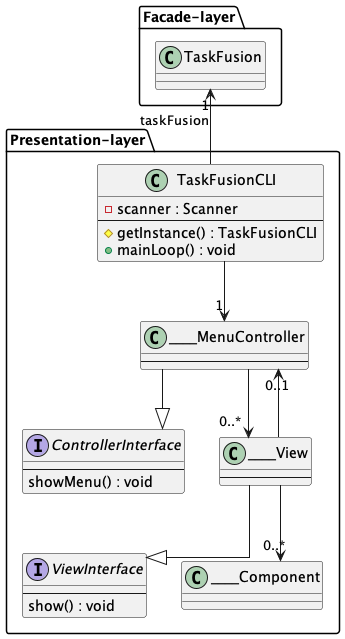
\includegraphics[width = 10cm, keepaspectratio]{TaskFusion/out/assets/diagrams/class_cli/TaskFusion-CLI.png}
    \label{fig:class_cli}
\end{figure}

\subsubsection{CLI brugergrænsefladen}
Da CLI grænsefladen til TaskFusion er opbygget af \textit{MenuController}'re og \textit{View}'s, ender vi da også med et netværk af mulige veje brugeren kan gå. For at få et overblik over TaskFusion, er herunder i \ref{fig:flow_cli} et \textit{flow}-diagram over menuer og sider i CLI grænsefladen.  
\begin{figure}[H]
    \centering
    \caption{Flowdiagram over CLI brugergrænsefladen}
    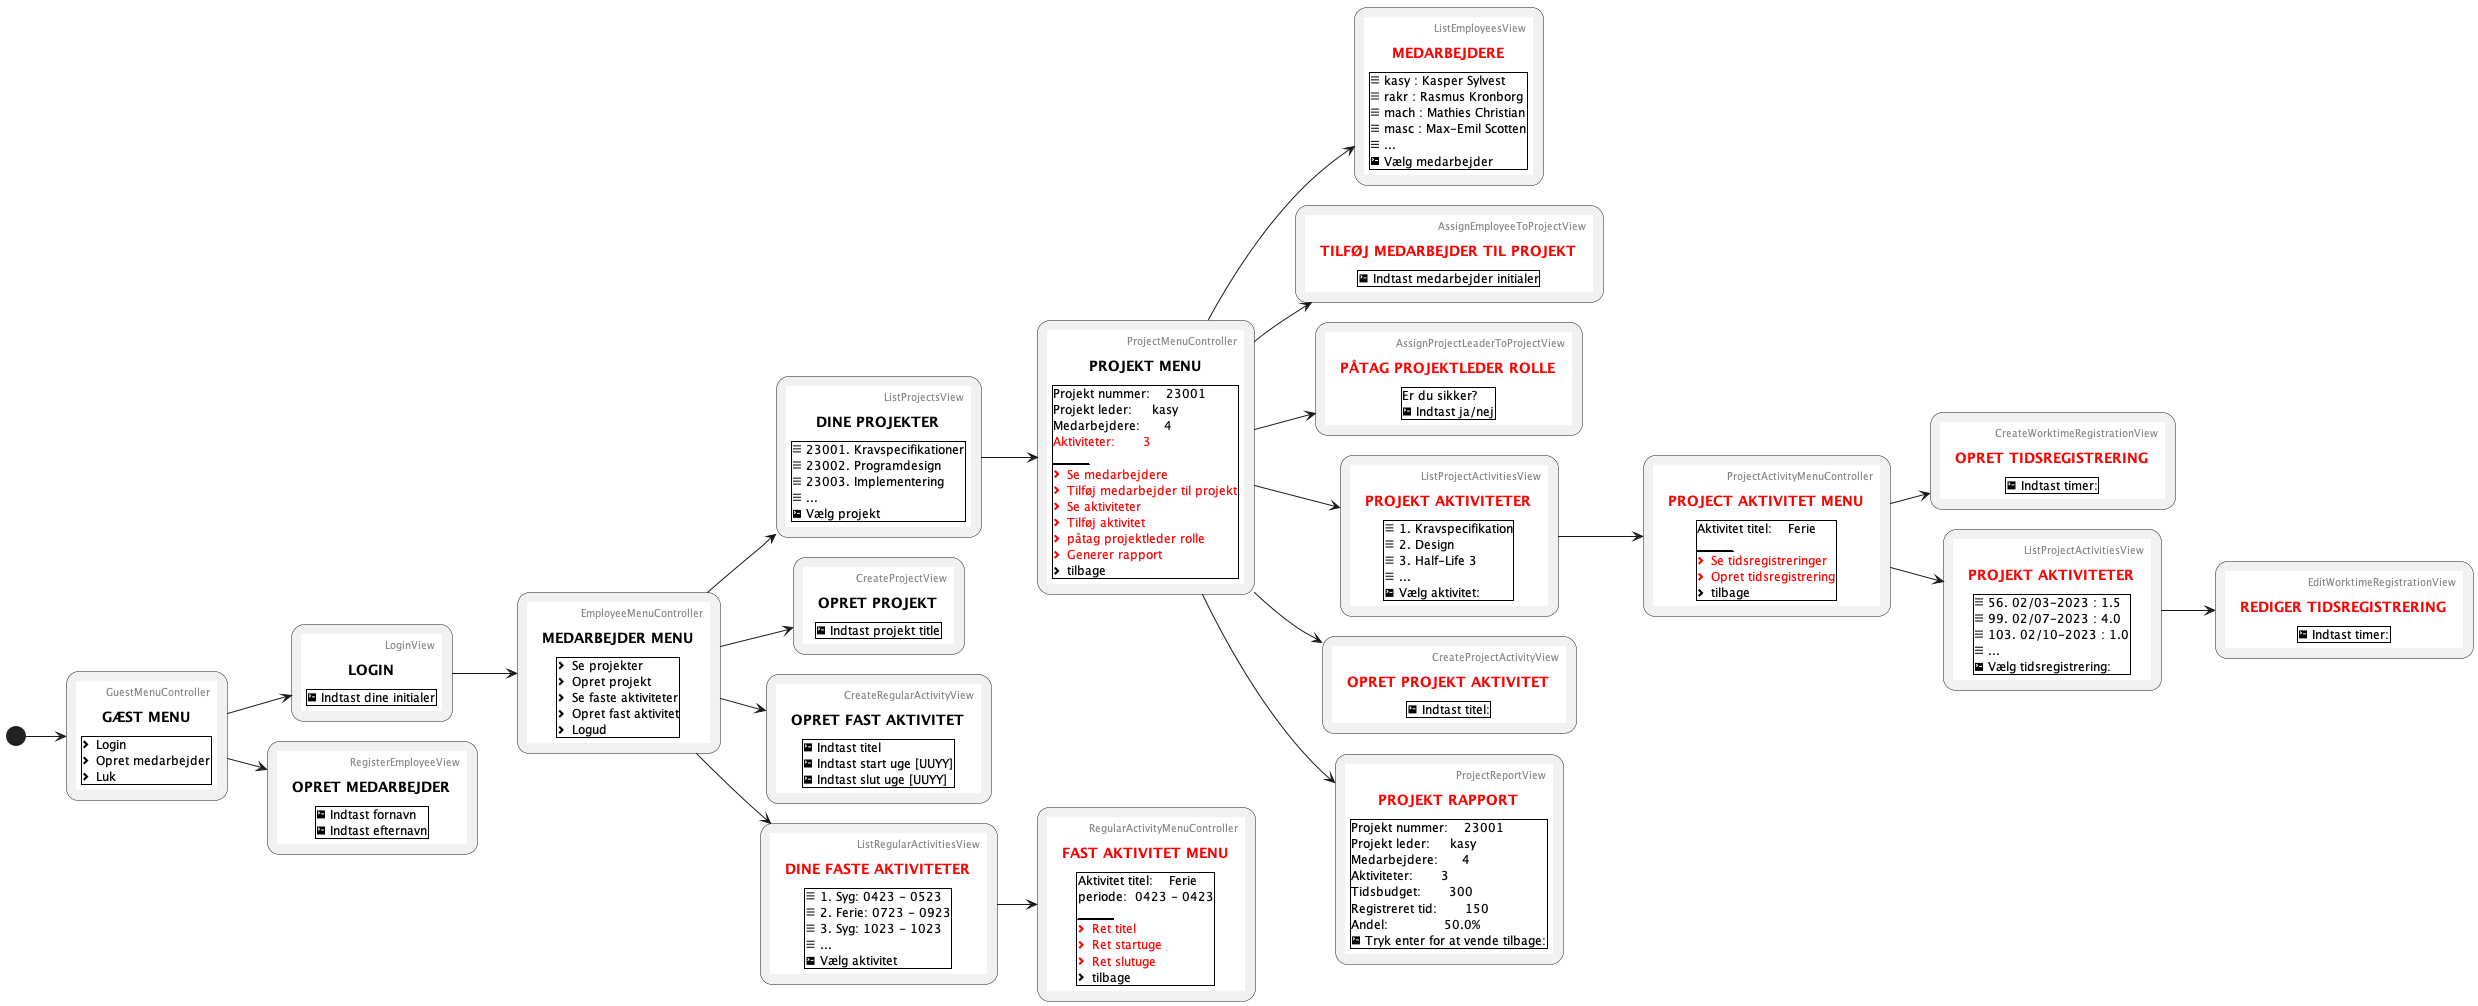
\includegraphics[width = \textwidth, keepaspectratio]{TaskFusion/out/assets/diagrams/flow_cli/flow_cli.png}
    \label{fig:flow_cli}
\end{figure}

